\chapter{COMBAT}

\begin{multicols}{2}

\section{ENCOUNTERS}

\index{Encounters}An encounter is, by definition, any significant event a character may happen upon.  An encounter can be hostile or non-hostile.  If an encounter turns hostile, it escalates into combat.  Combat lasts until one side is defeated, surrenders, retreats or the danger is otherwise no longer present.

\subsection{ENCOUNTER ACTIONS}

\index{Encounter Actions}There are several actions a party can take in an encounter.  Characters aren't limited to these options; these are just the more common choices.

Evade: The party avoids the encounter whether this means they ignore it, ride past it, or sneak around.  Hostile parties may pursue a fleeing party if they're aware of them.

Interact: The party interacts with the encounter by investigating or speaking in the case of intelligent creatures.

Fight: The party draws weapons and attacks.  

Wait: A party can specifically wait for a reaction.  Waiting is an action that increases the waiting party's next initiative roll by +1.  

\section{COMBAT}\index{Combat}

\subsection{TIME IN COMBAT}

\index{Combat!Time in Combat}Time in combat is measured in rounds, which equal a minute.  Ten rounds (or ten minutes) are called a turn.  Actions in combat are rarely simple exchanges.  Participants in combat are expected to defend against attacks, thrust, feint, and parry while trying to score a hit.

In general, characters can perform only one basic action per round.  The rest of their time is spent on smaller actions such as moving and dodging.  Basic actions include attacking, casting one spell, activating an item such as lighting a torch, moving full movement value, stabilizing a character, searching a body, grabbing a dropped item, bashing down a door, and drinking a potion. 

Some actions are so minor they require negligible time.  Examples are: speaking short sentences (rule of thumb is 20 words or less per character per round), drawing a weapon, removing a backpack or belt, falling prone or standing up.

Ultimately the GM has final say in what counts as a basic and minor action.
 
\subsection{COMBAT SEQUENCE}

\index{Combat!Combat Sequence}All combat follows four steps that repeat each round.

GM decides the actions of the monsters.

The PCs declare their actions and begin casting spells.

Initiative is rolled for all opposing parties.

Actions are resolved in order of initiative.

\paragraph{Step 1:}The GM determines, in secret, the actions of the NPCs.  If a spell is to be cast, he chooses it before the players announce their actions.

\paragraph{Step 2:} The players describe the actions their characters want to take including moving, attacking, and casting spells.  Actions can be general.  If a player says, ``I move and attack the nearest enemy" then his character will perform that action to the best of his ability.  If a spell is cast, then it begins in this phase and cannot be changed.  When the players are ready, the GM moves to step 3.

\paragraph{Step 3:} Initiative is rolled which determines which party goes first.

\paragraph{Step 4:} Actions are resolved based on initiative.  Attacks are made and spells with casting time less than 1 round are cast.  If initiative is a tie then all actions are simultaneous.

Some monsters, situations, or abilities may supersede the combat sequence.  

\subsection{COMBAT INITIATIVE}

\index{Initiative}Initiative is rolled each round during step 3.  An initiative roll is 1d10 for each opposing side.  Low initiative beats high and parties act in ascending order.  If the initiative of both sides is the same then compare the weapon's \index{Combat Speed}combat speeds and/or spell \index{Casting Time}casting times between two opponents to determine which attack or actions happen first.  There are also other several factors that may influence initiative rolls.  If the entire party doesn't qualify, then the individual members act on their new, modified initiative.

\noindent
\begin{minipage}{\columnwidth}

\captionof{table}{Initiative Modifiers}\label{initmods}
\noindent
\begin{tabular}{|p{0.72\columnwidth}|p{0.18\columnwidth}|}
\hline
Situation	& Modifier \\
\hline\hline
\rowcolor[gray]{.9}Hasted	& $-2$ \\
Slowed	& +2 \\
\rowcolor[gray]{.9}High ground	& $-1$ \\
Receive charge	& $-2$ \\
\rowcolor[gray]{.9}Knee deep water	&  +2\\
Slippery footing	& +2 \\
\rowcolor[gray]{.9}Waist deep water	& +4 \\
Underwater	& +6 \\
\rowcolor[gray]{.9}Hindered (climbing, tangled, held)	& +3 \\
Waiting	& +1 \\
\hline
\end{tabular}

\end{minipage}

\subsection{THE ATTACK ROLL}

\index{Attack Roll}\index{THACO}The act of attempting to strike a target, whether it's with a weapon or just tossing them an object to catch is considered an attack.  To make an attack your character must be capable of hitting his opponent (this means striking distance with most melee weapons).  The target's AC is subtracted from your character's THACO (giving a modified THACO). Then a d20 is rolled. Add or subtract all attack roll modifiers from the d20 roll, including those from Str and Dex.  If the modified d20 roll is equal to or greater than the modified THACO, the attack hits and \index{Damage}damage is rolled.

\subsection{ATTACK MODIFIERS}

\index{Attack Roll!Modifiers}\index{Combat!Attack Modifiers}Strength applies a modifier to hit with bows (but not crossbows) and melee weapons. Dexterity applies a modifier to hit with all bows and hurled weapons.  There is no limit to the modifiers added to an attack roll.  

Several situations may modify the attack roll.

\noindent
\begin{minipage}{\columnwidth}

\captionof{table}{Attack Roll Modifiers}\label{attackmods}
\noindent
\begin{tabular}{|p{0.66\columnwidth}|p{0.24\columnwidth}|}
\hline
Situation	& Modifier \\
\hline\hline
\rowcolor[gray]{.9}Attacker on higher ground	& +1 \\
Invisible opponent	& $-4$ \\
\rowcolor[gray]{.9}Opponent off-balance	& +2 \\
Helpless opponent (held, sleeping, paralyzed, etc.)	& Automatic* \\
\rowcolor[gray]{.9}Opponent stunned or prone	& +4 \\
Defender surprised	& +1 \\
\rowcolor[gray]{.9}Missile, long range	& $-5$ \\
Missile, medium range	& $-2$ \\
\rowcolor[gray]{.9}Rear attack	& +2 \\
\hline
\end{tabular}
\noindent\begin{tabular}{p{.98\textwidth}}
*In combat, a helpless opponent is struck automatically.  Outside of combat, a helpless opponent can be slain automatically. \\
\end{tabular}\vspace{.5em}

\end{minipage}

\subsection{MULTIPLE ATTACKS}

\index{Combat!Multiple Attacks}When a creature has multiple attacks as the result of multiple weapons (including the \index{Natural Attacks}natural weapons of animals or monsters), all attacks are rolled at the same time.  Multiple attacks using a single weapon, such as a fighter's attacks or firing a bow, are staggered.  The first attack is always made on the creature's initiative and the iterative attacks are made after every creature involved in combat has acted.  

If more than one creature is capable of multiple attacks then their iterative attacks occur according to initiative (but always after every other creature has acted).  Having an odd number of attacks are rolled differently; 3/2 is one attack in the first round and two in the second, 5/2 is two attacks in the first round and three in the second, 7/2 is three attacks in the first round and four in the second, and 9/2 is four attacks in the first round and five in the second.  

\subsection{FACING AND SPACE}

\index{Combat!Facing and Space}All combatants are assumed to have a front, flank, and rear.  Up to six attackers of equal size to the defender can attack.  For each size category larger than the defender, the attacker takes up one extra space.  For each size category smaller than the defender, the attacker takes up half the space.

\noindent
\begin{minipage}{\columnwidth}

\noindent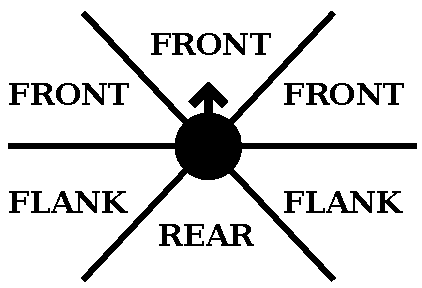
\includegraphics[width=\columnwidth]{facing.pdf}
\captionof{figure}{Facing}

\end{minipage}

Combatants will always keep their attackers in their front sights until they're overwhelmed.  Additional attackers fill up the front, flank, and rear in that order.  New attackers cannot attack a defender who's completely surrounded.  When fighting multiple opponents, the defender can switch his facing as he chooses.  Defenders cannot choose to face opponents they're unaware of.

\index{Armor Class!Effects of Facing}Characters attacked from the rear lose their dexterity bonus to AC and the attacker gains a +2 bonus to attack.

\subsection{WEAPON LENGTH}

The GM must decide if a character has adequate space to wield a weapon.  As a general rule, a combatant requires five-square-feet of space to wield a medium sized slashing or bludgeoning weapon and ten-square-feet of space to wield a large sized slashing or bludgeoning weapon.  Because they have no arcs, piercing weapons require very little space allowing multiple combatants to fight side-by-side.  
 
\subsection{CALLED SHOT}

Normally, characters don't target specific points when attacking their opponents.  The called shot is a maneuver that allows a character to specifically attack a point on a creature or target, such as the potion on their belt or hit a lock on a door latch without damaging the door itself.

\index{Attack Roll!Effects of Called Shots}A character making a called shot must announce their target before initiative is rolled and suffers a +1 penalty to their initiative.  Called shots apply a -4 penalty to the resulting attack roll.  If the attack succeeds, damage is rolled as normal.  Called shots deal the normal damage of the weapon regardless where it hits.  Called shots cannot be used to blind, maim, or cripple targets.  

\subsection{SPELL CASTING}

\index{Spell Casting}\index{Combat!Spell Casting}Casting a spell adds to the caster's initiative, delaying his action.  \index{Casting Time}If the casting time of a spell is less than 1 round (represented by a simple number in the casting time) then that number is added to the caster's initiative.  Spell casters begin casting before initiative is rolled and resolve on the caster's modified initiative (or at the end of the round or turn as the case may be for longer spells).  

Casters cannot move while casting spells and lose their dexterity bonus to AC, if any.  If a caster takes damage or fails a saving throw while casting a spell, his concentration is ruined causing the spell to fail and that casting to be wiped from his mind. 

\subsection{TWO WEAPON FIGHTING}

\index{Two-Weapon Fighting}\index{Combat!Two-Weapon Fighting}Only warriors and rogues may fight with two weapons.  The primary weapon can be any one-handed weapon.  The secondary weapon must be smaller in size and weight than the primary weapon, with the exception of daggers, knives, and dirks.  Any combination of two of these weapons can be used together.  A buckler may be used while fighting with two weapons, but no other shield is allowed, unless it is strapped to the back.  

Two weapon fighting allows a character an extra attack per round (1/1 becomes 2/1, 3/2 becomes 5/2, 5/2 becomes 7/2, etc.).  All characters are dominant in one hand of their choice (if checked randomly, there's a 10\% chance of being left-handed).  Attacking with two weapons applies a $-2$ penalty to attacks made with the weapon in the dominant hand and a $-4$ penalty to attacks made with the weapon in the non-dominant hand.  A positive dexterity---missile attack modifier reduces the penalties of two weapon fighting (to a maximum of +0 before other modifiers), while a negative dexterity---missile attack modifier increases the penalties of two weapon fighting.  Also refer to Combat Skills.

\subsection{ATTACKS WITH THE NON-DOMINANT HAND}

A character is assumed to use their dominant hand for all tasks such as using a weapon, so that if a character loses the ability to use their dominant hand, all actions performed by the non-dominant hand suffer a $-2$ penalty, modified by their dexterity---missile attack adjustment (to a maximum of +0 before other modifiers). 
 
\subsection{MOVEMENT IN COMBAT}

\index{Movement}\index{Combat!Movement}All combatants can move ten times their movement value in feet during a single round.

Combatants engaged in melee will turn to face their opponents if possible (see the section on facing for more details).  Combatants can block the movement of their targets if they both share the same movement type (someone fighting on the ground cannot block the movement of a flying creature).  Combatants cannot move through opponents unless they are able to push or knock them aside.

\subsection{MOVEMENT AND MELEE ATTACKS}

Combatants can move half their movement value in tens of feet and attack during the same round.  Attacking doesn't end the attacker's move unless the defender chooses to block the attacker's path or half of the attacker's movement value is reached.

\subsection{MOVEMENT AND RANGED ATTACKS}

Moving and firing missile weapons at the same time is difficult.  A combatant can move half their movement value in tens of feet and make a ranged attack at half their normal rate of fire rounded down.  If a weapon can only be fired once (such as with crossbows and most hurled weapons), increase the amount of rounds per attack by one.  For example, a person firing a short bow while moving would have an ROF of 1, a light crossbow would have an ROF of 1/2, and a heavy crossbow 1/3.

\subsection{CHARGE}

\index{Charge}A character can charge his opponent, increasing his movement value in tens of feet by 50\% and giving him a +2 bonus to his first melee attack.  \index{Armor Class!Effects of Charging}Charging gives the target a $-2$ bonus to his initiative roll (possibly allowing the target to move before the attacker moves), negates the attacker's dexterity bonus to AC, and inflicts a +1 penalty to the attacker's AC during the round the charge occurs.

\subsection{RETREAT}

\index{Retreat}There are two methods for retreating from combat; a careful withdrawal or haphazard fleeing.

\paragraph{Withdraw:} A character can carefully withdraw from an opponent that he is fighting in melee, while moving his full movement value in tens of feet.

\paragraph{Flee:} Fleeing means that a character drops all defenses to move as far away from his opponent as possible.  A fleeing character moves at his full, normal movement value in tens of yards.  When a character flees, all adjacent enemies can make as many melee attacks as they have in a given round against that fleeing character.  These attacks do not count against their normal limit per round and are made the instant their opponent turns to flee.

\subsection{NON-LETHAL COMBAT}

There are three kinds of non-lethal combat; brawling, wrestling, and overbearing.  Brawling means that a character uses his body to strike blows against the enemy, wrestling is a combination of grappling and holds, and overbearing is an attempt to drag an opponent down in a pin.

\subsection{BRAWLING AND WRESTLING}

\index{Brawling and Wrestling}Brawling occurs when characters attack with their primary appendages such as bare fists or feet.  Wrestling uses the entire body and both hands must be free.  When brawling or wrestling, an attack roll is made against the target's normal AC.  \index{Armor!Brawling and Wrestling}Wearing armor heavier than leather penalizes the attack roll while wrestling.

If the attack roll is successful, check the table for the result.  Brawling and wrestling can succeed on a roll of 1 although a 20 is always an automatic hit.

\paragraph{Brawl:} The type of blow is a descriptor and has no specific game effect.

\index{Damage!Brawling and Wrestling}\paragraph{Damage:} Brawling deals the listed damage per attack.  Metal gauntlets and the like increase damage to 1d3.  Strength applies to brawling damage.  25\% of the damage dealt is lethal and 75\% of damage dealt (minimum 1 point per attack) is non-lethal.  Non-lethal damage is recorded separately and any healing effect removes an equal amount of non-lethal and lethal damage.  If a creature is reduced to 0 HP while having non-lethal damage recorded, he immediately falls unconscious.  A brawler can pull his attacks, dealing no lethal damage, but the \%KO still applies.

\index{Knockout!Brawling and Wrestling}\paragraph{\%KO:} Each successful attack has a chance to KO the victim.  If successful, the victim is stunned for 1d10 rounds.

\paragraph{Wrestle:} Wrestling moves marked with an asterisk are holds that can be maintained until broken (no further attack roll necessary).  A hold is broken by a throw, gouge, or assistance by another character, or attack with a melee weapon.  All wrestling moves inflict 1 point of damage plus strength bonus (attacker's choice to add in strength).  A hold deals a cumulative 1 point of damage per round held.

\noindent
\begin{minipage}{\columnwidth}

\captionof{table}{Brawling and Wrestling}\label{brawlwrestle}
\noindent
\begin{tabular}{|p{0.06\columnwidth}|p{0.24\columnwidth}|p{0.13\columnwidth}|p{0.08\columnwidth}|p{0.24\columnwidth}|}
\hline
Roll	& Brawl	& Damage	& \%KO	& Wrestle \\
\hline\hline
\rowcolor[gray]{.9}20+	& Haymaker		& 2	& 10	& Bear hug* \\
19	& Back kick		& 0	& 1		& Arm twist \\
\rowcolor[gray]{.9}18	& Rabbit punch	& 1	& 3		& Kick \\
17	& Kidney punch	& 1	& 5		& Trip \\
\rowcolor[gray]{.9}16	& Front kick	& 1	& 2		& Elbow smash \\
15	& Jab			& 2	& 6		& Arm lock* \\
\rowcolor[gray]{.9}14	& Uppercut		& 1	& 8		& Leg twist \\
13	& Crescent kick	& 2	& 10	& Leg lock \\
\rowcolor[gray]{.9}12	& Roundhouse	& 1	& 5		& Throw \\
11	& Hook			& 2	& 10	& Gouge \\
\rowcolor[gray]{.9}10	& Back fist		& 1	& 3		& Elbow smash \\
9	& Combination	& 1	& 10	& Leg lock* \\
\rowcolor[gray]{.9}8	& Reverse kick	& 1	& 9		& Headlock* \\
7	& Combination	& 2	& 10	& Throw \\
\rowcolor[gray]{.9}6	& Side kick		& 2	& 8		& Gouge \\
5	& Overhand		& 1	& 3		& Kick \\
\rowcolor[gray]{.9}4	& Cross			& 2	& 5		& Arm lock* \\
3	& Hook			& 2	& 12	& Gouge \\
\rowcolor[gray]{.9}2	& Uppercut		& 2	& 15	& Headlock* \\
1	& Glancing blow	& 0	& 2		& Leg twist \\
\rowcolor[gray]{.9}\textless 1	& Wild swing	& 2	& 25	& Bear hug* \\
\hline
\end{tabular}
\noindent\begin{tabular}{p{.98\textwidth}}
*Holds are maintained each round until broken \\
\end{tabular}\vspace{.5em}

\end{minipage}

\noindent
\begin{minipage}{\columnwidth}

\captionof{table}{Armor Modifiers for Wrestling}\label{wrestlingarmor}
\noindent
\begin{tabular}{|p{0.66\columnwidth}|p{0.24\columnwidth}|}
\hline
Armor	& Mod. \\
\hline\hline
\rowcolor[gray]{.9}Studded leather	& $-1$ \\
Chain, ring, scale mail	& $-2$ \\
\rowcolor[gray]{.9}Banded, splint, plate	& $-5$ \\
Field plate	& $-8$ \\
\rowcolor[gray]{.9}Full plate	& $-10$ \\
\hline
\end{tabular}

\end{minipage}
 
\subsection{OVERBEARING}

\index{Overbearing}Overbearing attempts to drag an opponent and pin them to the ground.  \index{Attack Roll!Overbearing}An attack roll is made against the target.  Each difference in size between the attacker and defender modifies the attack roll by 4 (+4 for each size the attacker is larger than his opponent and $-4$ for each size that the attacker is smaller than his opponent).  An attacker suffers a $-2$ penalty for each number of legs beyond two the defender has.  A defender has no penalty if it has no legs such as with amorphous opponents.

If the attack succeeds, the opponent is pulled down.  A character can be pinned if another successful overbear attack is made.  For each attacker beyond one, a +1 modifier is added.  The weakest attacker in a group makes the actual attack and modifiers are added for the largest attacker in a group.

\subsection{WEAPONS AND NON-LETHAL COMBAT}

\index{Combat!Non-lethal Combat}\paragraph{Weapons in Defense:} Brawling, wrestling, or overbearing an opponent armed with a weapon enables them to one immediate, free attack with a +4 bonus.  When wrestling, characters may attack each other with small weapons.

\paragraph{Non-lethal Weapon Attacks:} Slashing and piercing weapons can be used to deal \index{Damage!Non-lethal}non-lethal damage.  Ranged attacks, thrown or fired, cannot be used to non-lethally.  \index{Attack Roll!Non-lethal Combat}Attacking non-lethally applies a $-4$ penalty to the attack roll and 50\% of the damage dealt is non-lethal.

\subsection{TOUCH SPELLS AND COMBAT}

\index{Combat!Spell Casting}A spell caster can simply touch his target as part of casting their spell.  There are two exceptions to this rule.  Most touch spells are only effective for the round they're cast (a missed attack results in the spell fizzling), however, some allow the caster to make multiple touch attacks.

\index{Armor Class!Touch Spells}\index{Attack Roll!Touch Spells}\paragraph{Unwilling Targets:} The caster must make a successful attack roll against AC 10 modified only by dexterity and magical bonuses.  Wearing +1 plate mail will provide a $-1$ bonus to AC, wearing +3 leather will offer $-3$ bonus to AC, and bracers, rings, cloaks, etc. provide normal bonuses.

\paragraph{Willing Targets:} Touching a willing target is automatic so long as both characters aren't engaged in melee.  To hit a willing target performing any action other than waiting for the spell, the caster must hit an AC of 10.  

\subsection{RANGED ATTACKS}

\index{Missile Combat}Ranged weapon attacks are similar to melee attacks.  Strength modifiers are applied to the damage rolls of hurled weapons, and in some cases strength modifiers can be applied to both damage and attack rolls of bows.  Dexterity modifiers are also applied to the attack roll of all ranged weapons relying on the attacker's aim.  A weapon's rate of fire is handled as a multiple attack.  Most ranged weapons fire in a straight line although they can be fired in an arc.  Calculate the additional range it takes to fire a weapon in an arc.  Some weapons can only be fired in an arc and as such have a minimum range to work.  
 
\subsection{COVER AND CONCEALMENT}

\index{Cover and Concealment}Defenders can use cover and concealment to protect against ranged attacks.  Concealment is any object that hides a character but doesn't block missile attacks such as a bush or tapestry.  Cover is any object that hides and protects a character such as a wall or furniture.  Cover and concealment apply the following penalties to an attacker's ranged attack.

Cover (but not concealment) grants the modifier as a bonus to the defender's saving throw against spells or effects that cause damage like a \textit{fireball} or dragon's breath.  A character with 90\% or more cover suffers one-half normal damage on a failed save and no damage on a successful save.  This assumes the defender's cover blocks the spell's effect; for example, a \textit{fireball} would have full effect if it exploded behind the cover.

\noindent
\begin{minipage}{\columnwidth}

\captionof{table}{Cover/Concealment Modifiers}\label{covermods}
\noindent
\begin{tabular}{|m{0.37\columnwidth}|m{0.24\columnwidth}|m{0.24\columnwidth}|}
\hline
Target's Position	& \multicolumn{2}{c|}{Modifier} \\
&	Cover	& Concealment \\
\hline\hline
\rowcolor[gray]{.9}25\% hidden	& $-2$	& $-1$ \\
50\% hidden	& $-4$	& $-2$ \\
\rowcolor[gray]{.9}75\% hidden	& $-7$	& $-3$ \\
90\% hidden	& $-10$	& $-4$ \\
\hline
\end{tabular}

\end{minipage}

\subsection{FIRING INTO CROWDS}

Firing into crowds has a chance to hit a random target.  Having a clear shot (such as having the high ground) eliminates this chance. 

Under normal circumstances, the character using the missile weapon chooses a target in the crowd and rolls an attack with all normal modifiers. If the modified attack roll is too low to hit the armor class of the chosen target or any creatures or characters (including allies) adjacent to the chosen target, it is simply counted as a miss.  If the attack roll is high enough to be successful versus the armor class of the chosen target or any creatures or characters (including allies) adjacent to the chosen target, the GM must assign a number to the chosen target, and each adjacent creature, based on its size.  Small and smaller creatures count as 1, medium creatures 2, large as 3, huge as 8, gargantuan as 12, and colossal as 16 each.  Add these numbers together. Each creature is then assigned a percentage chance by dividing its numerical rating by the total.  This randomly rolled target's AC is then compared to the original modified attack roll to see if the hit was successful.  Damage is rolled and modified normally whether friend or foe is struck.  

Otherwise, a called shot is required to guarantee that only the chosen target will be struck.  This called shot is made at $-6$ to hit, plus appropriate penalties for cover or concealment that the ``crowd" provides to the target; loyal bodyguards may attempt to block incoming missiles (providing the equivalent of cover), while the character's allies may attempt to dodge at the right moment (providing the equivalent of concealment).  If the called shot misses, assume it misses everyone.

For example, a human worth 2 points and AC 2 and a halfling worth 1 point and AC 7 are in melee combat with a kobold also worth 1 point and AC 7. An elf fires an arrow into the melee and rolls high enough to hit the halfling or kobold, but not the human. The GM adds up the numerical values. In this case, 2~+~1~+~1 =4.  So it follows that the arrow is 50\% likely (2/4) to bounce off the human's heavy armor (thereby missing everyone), 25\% likely (1/4) to hit the halfling and 25\% likely (1/4) to hit the kobold. If the elf tried a called shot against the kobold, the GM would determine the kobold to be under 75\% concealment (since allies are surrounding the target), thus giving a total of $-9$ to hit the kobold.  If, instead of a kobold, the human and halfling were in melee with an ogre, the total would be 2~+~1~+~3 = 6, thus reducing the human's chance to 33\% or 2/6, the halfling's chance is then 17\% or 1/6, and the ogre's chance is 50\% or 3/6.  If the elf tried a called shot against the ogre, the GM would determine the ogre to be under 50\% concealment ($-8$ penalty to hit).  Finally, a kobold spell caster targeted by the elf, but surrounded by three ogre body guards, would have only a 10\% chance of being the actual target, while each of the ogres would have a 30\% chance to be the target instead.  If the elf tried a called shot against this kobold, the GM would determine that the kobold is under 90\% cover and apply a $-16$ penalty.  The GM will have to adjudicate the cover or concealment penalty for called shots in cases where allies and enemies are mixed.

\subsection{INDIRECT MISSILES}

\index{Indirect Missiles}An indirect missile is any ranged weapon that targets a specific point, not a creature.  Indirect missiles generally shatter when they hit their target, but the GM may rule that they receive a saving throw to resist breaking.  Indirect missiles of five pounds or less can be thrown with a short range of 10 feet, medium range of 20 feet, and long range of 30 feet; heavier items have reduced ranges based on the GM's decision.  In general, trying to throw an item heavier than one-third of a character's strength---max weight score requires a successful bend bars check.  Some weapons, like the staff sling and catapult, can be used to fire indirect missiles using the range of the weapon. 

To use an indirect missile, an attack is made against an AC 10 to target a specific point (not a creature).  Penalties may apply especially in situations where the target isn't visible or has cover.  If the attack misses the intended point, it hits in a random location.   Creatures or characters in this random location are now subject to the missiles effects.  An indirect missile attack that fails from short-range falls 1d6 feet away from the intended target, from medium-range, the missile falls 1d10 feet away from the intended target, and from long-range, the missile lands 2d10 feet away from the intended target.  Roll 1d10 and consult the scatter diagram to determine the direction the missile falls.

All creatures standing in the effective area take a direct hit and damage is dealt based on the missile.  Unless noted, all indirect missiles deal splash damage to anything standing within 3' of the effective area.

\noindent
\begin{minipage}{\columnwidth}

\noindent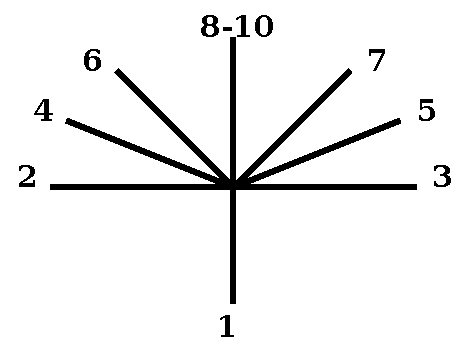
\includegraphics[width=\columnwidth]{scatter.pdf}
\captionof{figure}{Scatter Diagram}

\end{minipage}

\noindent
\begin{minipage}{\columnwidth}

\captionof{table}{Indirect Missile Effects}\label{covermods}
\noindent
\begin{tabular}{|m{0.22\columnwidth}|m{0.21\columnwidth}|m{0.23\columnwidth}|m{0.14\columnwidth}|}
\hline
Type	& Effective Area	& Direct Hit	& Splash \\
\hline\hline
\rowcolor[gray]{.9}Acid	& 1' diameter	& 2d4 HP	& 1 HP \\
Holy water	& 1' diameter	& 2d3 HP	& 2 HP \\
\rowcolor[gray]{.9}Greek fire	& 3' diameter	& 2d6/1d6 HP	& 1d3 HP \\
Poison	& 1' diameter	& special	& special \\
\hline
\end{tabular}

\end{minipage}

\subsection{TYPICAL INDIRECT MISSILES}

\index{Acid}\paragraph{Acid:} Acid damage cannot be healed by regeneration.  For characters that can regenerate, calculate acid damage separately.

\index{Holy Water}\paragraph{Holy Water:} Deals damage to most undead and evil creatures from the lower planes.  Unholy water deals damage to paladins and good creatures from the upper planes.  Holy and unholy water deal damage like acid (cannot be regenerated) and have no affect on gaseous creatures or those otherwise without a material form.

\index{Oil}\paragraph{Oil:} Damages a creature only when lit.  Typical use involves an attack that splashes an area with oil and a second attack that drops a lit torch or other object in the area.  A `Molotov cocktail' (flammable liquid in a fragile container with a cloth attached to the open end) can be constructed in one round, lit in the second round (using flint and steel), and thrown in the third round.  A burning object like a torch allows a cocktail to be lit and thrown in a same round.

\index{Poison}\paragraph{Poison:} Most poisons are liquid or powder and only work on a direct hit. Therefore, they have no effective splash damage.  Poisonous gasses, however, cause the same outcome to those within the area of a direct hit and those receiving only splash damage.

\subsection{HEAVY OBJECTS AS MISSILE WEAPONS}

Heavy objects like hurled boulders or iron balls roll when they strike the ground and do not shatter.  An attack roll is made to hit a location as a normal indirect missile (AC 10), but scatter distance, in the case of a missed attack, is doubled.  Any creature standing where a heavy object hits takes direct damage.  After hitting the ground, heavy objects bounce along their intended path for 3d10 feet before coming to a halt.  This range may be halved if going up hill or doubled going downhill.  

If the heavy object travels through a space occupied by a creature, make an attack roll against that creature with a $-2$ penalty for each 10' the heavy object bounced.  If the targets are in a tight formation or in an area where movement is restricted (GM decides), all targets in the heavy object's path are automatically hit and take direct damage.  To determine scatter damage, subtract the distance the heavy object rolled from the damage dealt on a direct hit.

\section{SAVING THROWS}

\index{Saving Throws}Saving throw represents a chance to avoid or reduce a harmful effect.  Saving throws are instinctive, thus a character that isn't even aware of the danger can react to it.  To make a saving throw, a character rolls 1d20 plus applicable modifiers and succeeds by equaling or exceeding his save score for that type of effect.  Each character has specific saving throws based on their class and level.  

\subsection{SAVING THROW PRIORITY}

\index{Saving Throws!Saving Throw Priorities}Most spells and effects specify which save to make, but in cases where saving throws aren't clear (such as an effect falling under two different kinds of saves), the saving throw is determined in order of priority from `save vs. paralyzation, poison, or death' to `save vs. spell'.  For example, a poison effect from a wand would require a `save vs. poison' because it has the highest priority, despite also being a spell cast from a wand, which would normally require a `save vs. wands' or a `save vs. spell'.

\paragraph{Save vs. Paralyzation, Poison, or Death:} Resists effects caused by poison, a paralyzing attack, spells designed to kill the character outright, and attacks that require great will power or physical fortitude to resist.  

\paragraph{Save vs. Rod, Staff, or Wand:} Resists effects caused by magical implements such as a rod, staff, or wand.  Can also be used to save against unusual sources of magic such as magical terrain.

\paragraph{Save vs. Petrification or Polymorph:} Resists effects that create a permanent or temporary physical change in the subject such as petrification or polymorph.

\paragraph{Save vs. Breath Weapon:} Resists affects that may be avoided by manual dexterity and agility, like a dragon's breath attack, falling objects, or maintaining balance on a slippery floor.

\paragraph{Save vs. Spell:} Resists the magical attacks of a spell caster or item, provided no other type of save is more appropriate.  Save vs. spell is also used to resist any effect that doesn't have a definite classification.

\subsection{CREATURES AND SAVING THROWS}

Creatures and NPCs without ability scores normally use the warrior's saving throw progression based on hit dice.  Creatures who can cast either wizard or cleric spells use the appropriate spell caster's saving throw progression, and those with thief abilities use the thief's saving throw progression.

\subsection{VOLUNTARILY FAILING SAVING THROWS}

By default, a character always attempts to resist potential effects. However, a character can choose to purposefully fail a saving throw.  This is a conscious decision that must be clearly stated.  Voluntarily failing causes the effect to work as normal.

\subsection{ABILITY CHECKS AS SAVING THROWS}

\index{Ability Check!as Saving Throw}When a character can avoid damage through the use of an ability score, an ability check is made instead of a save.  A character that falls down a cliff might be allowed a strength check to jam his pick into the wall or a dexterity check to land properly when he hits the ground to reduce the damage.

\subsection{MODIFYING SAVING THROWS}

Magical items, specific rules, and unusual situations can directly modify the saving throw roll.  Bonuses and penalties modify the die roll, not the saving throw required.  

\index{Ability Scores!Modifying Saving Throws}\paragraph{Ability Scores:} \index{Wisdom!Saving Throw Modifiers}High wisdom gives a bonus to save vs. enchantments, illusions, and other mental effects.  \index{Constitution!Saving Throw Modifiers}Extremely high Constitution provides bonuses to saves versus poison, \index{Dexterity!Saving Throw Modifiers}and high dexterity gives a bonus to save vs. attacks that can be avoided by quick movement like a \textit{fireball} or breath weapon.  Low scores often apply penalties.

\paragraph{Magical items:} Some magical items like cloaks and rings give bonuses to saves as mentioned in their description.

\paragraph{Magical Armor:} The enchantment bonus of magical armor gives a bonus against spells and effects that deal damage to the external parts of the body such as fire, damage-causing spells, disintegration, and falling.  It does not protect against gas, poison, mental abilities or any other effects that don't inflict physical damage.

\paragraph{Specific spells, poisons, or items:} Certain spells or items automatically carry a modifier to the character's save.  Potent spells may carry a penalty, while spells easily resisted carry bonuses.  Some poisons, particularly mild ones like from an insect, grant a bonus to save because they're not particularly deadly.

\paragraph{Special Situations:} In cases where an effect should be easier or more difficult to save against, the GM sets the modifier.  As a general rule, saving throw modifiers should range between $-4$ and +4.  A $-4$ penalty represents an extreme or powerful effect while +4 bonus represents a completely favorable situation or weak effect.
 
\section{MAGIC RESISTANCE}

\index{Magic Resistance}Magic resistance is an innate ability to resist the effects of spells.  It requires no conscious effort from the creature to work and is always considered ``on".  It cannot be imparted to other characters, unless a special power allows it to be.  Magic resistance is given as a percentile; if the roll is equal to or lower than the percentile the magic is resisted.  If the magic resistance fails, then the spell affects the target as normal including rules on saving throws.

Magic resistance protects creatures against direct spells and spell-like powers (including beneficial ones), unless the creature purposely decides to lower it.  It does not protect against magic weapons or the natural results of a spell, such as objects falling on a target as the result of \textit{earthquake}.  

Succeeding against a magic resistance check can have several different results depending on the nature of the spell.

\paragraph{Targeted Spells:} Each individual creature with magic resistance makes a check to resist the effect.  If only a single target is designated and the target makes its check, or all targets make their check, the spell fails completely.

\paragraph{Area Effect Spells:} These spells affect a single point.  The spell effect goes off as normal but the targeted creature is unaffected if they succeed on their check.

\paragraph{Continuous Spells:} These spells affect the target when they pass through such as magical hexes or circles.  Magic resistance only comes into effect if the creature is targeted as a result of the spell.  Normally a continuous spell isn't instantly negated by a successful magic resistance check, however, the GM may rule otherwise.

\paragraph{Permanent Spells:} Magic resistant creatures are unaffected by permanent spells in their effective area for the duration they remain in the spell area.  A magic resistant creature never negates permanent spells.

\section{IMMUNITY TO WEAPONS}

\index{Weapon Immunity}Some monsters are immune to the damage of normal weapons.  A monster immune to weapon damage is visibly wounded but suffers no pain (damage to hit points) from the attack.  Magical effects imparted by the weapon, such as fire or poison, still take effect.

The two most common forms of weapon immunity can be bypassed by magic weapons or silvered weapons.  Magic weapons must have an enchantment bonus that matches or is greater than the creature's listed immunity.  Only weapons forged completely from silver can damage creatures weak against silver.

For the purposes of overcoming weapon immunity, the \index{Natural Attacks}natural attacks of monsters can act as magical weapons. This ability does not extend to NPC or Player Character humans or demi-humans.  Consider a creature's attacks to be a magic weapon based on its HD.  With some exceptions, the attack itself is not actually magical so the creature's attack and damage rolls are not modified.

\noindent
\begin{minipage}{\columnwidth}

\captionof{table}{Monster Hit Dice Overcoming Immunity}\label{overcomingimmunity}
\noindent
\begin{tabular}{|p{0.42\columnwidth}|p{0.48\columnwidth}|}
\hline
Hit Dice	& Overcomes \\
\hline\hline
\rowcolor[gray]{.9}4	& +1 weapon \\
6	& +2 weapon \\
\rowcolor[gray]{.9}8	& +3 weapon \\
10	& +4 weapon \\
\hline
\end{tabular}

\end{minipage}

\end{multicols}

\noindent
\begin{minipage}{\columnwidth}

\captionof{table}{Turn Undead}\label{turnundead}
\noindent
\begin{tabular}{|p{0.116\textwidth}|p{0.048\textwidth}|p{0.048\textwidth}|p{0.048\textwidth}|p{0.048\textwidth}|p{0.048\textwidth}|p{0.042\textwidth}|p{0.042\textwidth}|p{0.042\textwidth}|p{0.042\textwidth}|p{0.060\textwidth}|p{0.060\textwidth}|p{0.049\textwidth}|}
\hline
Undead HD	& 1	& 2	& 3	& 4	& 5	& 6	& 7	& 8	& 9	& 10--11	& 12--13	& 14+ \\
\hline\hline
\rowcolor[gray]{.9}Under 1 HD	& 10	& 7	& 4	& T	& T	& D	& D	& D*	& D*	& D*	& D*	& D* \\
1 HD	& 13	& 10	& 7	& 4	& T	& T	& D	& D	& D*	& D*	& D*	& D* \\
\rowcolor[gray]{.9}2 HD	& 16	& 13	& 10	& 7	& 4	& T	& T	& D	& D	& D*	& D*	& D* \\
3 HD	& 19	& 16	& 13	& 10	& 7	& 4	& T	& T	& D	& D	& D*	& D* \\
\rowcolor[gray]{.9}4 HD	& 20	& 19	& 16	& 13	& 10	& 7	& 4	& T	& T	& D	& D	& D* \\
5 HD	& --	& 20	& 19	& 16	& 13	& 10	& 7	& 4	& T	& T	& D	& D \\
\rowcolor[gray]{.9}6 HD	& --	& --	& 20	& 19	& 16	& 13	& 10	& 7	& 4	& T	& T	& D \\
7 HD	& --	& --	& --	& 20	& 19	& 16	& 13	& 10	& 7	& 4	& T	& T \\
\rowcolor[gray]{.9}8 HD	& --	& --	& --	& --	& 20	& 19	& 16	& 13	& 10	& 7	& 4	& T \\
9 HD	& --	& --	& --	& --	& --	& 20	& 19	& 16	& 13	& 10	& 7	& 4 \\
\rowcolor[gray]{.9}10 HD	& --	& --	& --	& --	& --	& --	& 20	& 19	& 16	& 13	& 10	& 7 \\
11+ HD	& --	& --	& --	& --	& --	& --	& --	& 20	& 19	& 16	& 13	& 10 \\
\rowcolor[gray]{.9}Special**	& --	& --	& --	& --	& --	& --	& --	& --	& 20	& 19	& 16	& 13 \\
\hline
\end{tabular}
\noindent\begin{tabular}{p{.98\textwidth}}
*2d4 additional creatures of this type are turned. \\
**Special undead include unique monsters greater than 11 hit dice, undead on the negative material plane, or undead native to the outer planes regardless of hit dice. \\
\end{tabular}\vspace{.5em}

\end{minipage}

\begin{multicols}{2}

\section{SPECIAL ATTACKS}

\subsection{TURN UNDEAD}

\index{Turn Undead}Priests and paladins can turn undead, however, druids cannot.  Turning is the act of exerting divine power through a holy object to scare away or destroy undead. For the purposes of turning undead, a paladin is considered a priest two levels lower than his actual level.

Turning requires a holy object (usually a symbol of their deity or a blessed object) and can be used once per encounter, although multiple priests can use it at once.  Turning counts as a hostile action and takes effect on the priest's initiative.  Both hands must be free (except for the one holding the holy symbol) and the priest must clearly speak and present his symbol.  All undead able to see the priest are affected. 

Cross check the HD of the undead (down the side) against the priest's level (across the top) and, if a number is listed, roll 1d20.  If the number is greater than or equal to the target number in the column the attempt is successful.  ``T" stands for turned, ``D" stands for dispel (the targeted undead is instantly destroyed), and ``--" means the priest of that level cannot turn the listed undead.  Only one die is rolled regardless of the number of undead and each type is affected individually.

If the turn is successful then it affects 2d6 undead.  If the undead are mixed then the lowest hit dice undead are targeted first.  Turned undead retreat until out of sight of the priest that turned them; the mindless undead remain hiding there, but intelligent undead generally only hide until they're certain the priest has passed and may attempt to attack again.  If they cannot complete this, they circle at a distance no closer than 10 feet.  If the priest forces the undead closer then the turning is immediately broken and the undead behave normally.

Turning lasts as long as the priest maintains his concentration (no rolls are needed).  He can perform complex actions, such as attacking or casting spells, but must remain aware of the undead he turned and maintain a hold on his holy symbol. 

\subsection{DOMINATE UNDEAD}

\index{Turn Undead!Dominate Undead}Evil priests do not turn undead but dominate them.  An evil priest is bound by the same restrictions as a normal priest, but instead of turning an undead, they can command them.  A successful turning check (or a ``T") results in the undead following the first order given until completion, after which point it's no longer beholden to the priest.  A ``D" means the undead is completely subservient to the evil priest.  An evil priest can command up to 12 undead at a time.

Evil priests can also turn paladins, but the attempt is made at three levels lower than their actual level.  For example, an 8\textsuperscript{th} level evil priest would be considered only 5\textsuperscript{th} level.  A turned paladin is filled with negative energy and is forced to flee from the sight of the evil priest.  A result of ``D" is handled as a turn, or ``T".

\subsection{CHARMED CREATURES}

\index{Charmed Creatures}Charmed creatures can be given orders by the caster.  In the event the player characters \textit{charm} a monster, they can direct it to attack.  Charmed monsters will fight with their normal weapons but will not use their special abilities unless directly commanded to do so.  Likewise, if a player character is charmed, the GM must use whatever attack forms the caster knows his target possesses.  

Charming a spell caster is dangerous.  While a charmed spell caster can tell his master what spells he has memorized, there's a 25\% chance that the charmed spell caster will cast a spell that's harmful to himself and his master.

 
Charmed creatures cannot carry out actions requiring personal judgment.  Orders given must be distinct and precise, although charmed creatures do not actively try to circumvent or distort orders.  Charmed creatures refuse to obey self-destructive orders, such as committing suicide, but since combat has many variables, it's not considered self-destructive, even against impossible odds.

Monsters with charm powers (like vampires) require no verbal communication.  All orders are given mentally.  Spells that charm creatures require some means of verbal communication and a shared language, however, hand gestures and body language can be used to convey simple phrases such as ``I'm injured" and ``Go there."

\subsection{GAZE ATTACKS}

\index{Gaze Attacks}Some creatures have the ability to cause effects simply by gazing into their opponent's eyes.  All characters are considered to be looking at their opponent in a fight and suffer the effects of the gaze each round.  Attacking a creature's rear allows the attacker to avoid the creature's gaze.  Creatures with gaze attacks can choose to avoid looking in their opponent's eyes, negating their gaze attack.

Characters can choose to avert their eyes by only looking in the general direction of their target.  There's a 20\% chance each round that a character averting his eyes will still accidentally meet the gaze of his opponent.  Characters can completely avoid the gaze of a creature simply by looking at the ground or closing their eyes, however, they're considered blinded while attacking the opponent.  Finally, characters can fight while looking through a mirror or reflective surface.  Holding a mirror requires an empty hand.  The wielder suffers a $-2$ penalty to attack rolls loses his dexterity bonus to AC.

\end{multicols}

\noindent
\begin{minipage}{\columnwidth}

\captionof{table}{Item Saving Throws}\label{itemsaves}
\noindent
\begin{tabular}{|p{0.120\textwidth}|p{0.053\textwidth}|p{0.072\textwidth}|p{.096\textwidth}|p{0.053\textwidth}|p{0.083\textwidth}|p{0.060\textwidth}|p{0.060\textwidth}|p{0.083\textwidth}|p{0.083\textwidth}|}
\hline
Item	& Acid	& Crush\-ing	& Disin\-tegrate	& Fall	& Magic Fire	& Fire	& Cold	& Lightning	& Electricity \\
\hline\hline
\rowcolor[gray]{.9}Bone, Ivory		& 11	& 16	& 19	& 6	& 9	& 3	& 2	& 8	& 2 \\
Cloth			& 12	& --	& 19	& --	& 16	& 13	& 2	& 18	& 2 \\
\rowcolor[gray]{.9}Glass			& 5	& 20	& 19	& 14	& 7	& 4	& 6	& 17	& 2 \\
Leather			& 10	& 3	& 19	& 2	& 6	& 4	& 3	& 13	& 2 \\
\rowcolor[gray]{.9}Metal			& 13	& 7	& 17	& 3	& 6	& 2	& 2	& 12	& 2 \\
Oils*			& 16**	& --	& 19	& --	& 19	& 17	& 5	& 19	& 16 \\
\rowcolor[gray]{.9}Paper			& 16	& 7	& 19	& --	& 19	& 19	& 2	& 19	& 2 \\
Potions*		& 15**	& --	& 19	& --	& 17	& 14	& 13	& 18	& 15 \\
\rowcolor[gray]{.9}Pottery			& 4	& 18	& 19	& 11	& 3	& 2	& 4	& 2	& 2 \\
Rock, Crystal	& 3	& 17	& 18	& 8	& 3	& 2	& 2	& 14	& 2 \\
\rowcolor[gray]{.9}Rope			& 12	& 2	& 19	& --	& 10	& 6	& 2	& 9	& 2 \\
Wood, thick		& 8	& 10	& 19	& 2	& 7	& 5	& 2	& 12	& 2 \\
\rowcolor[gray]{.9}Wood, thin		& 9	& 13	& 19	& 2	& 11	& 9	& 2	& 10	& 2 \\
\hline
\end{tabular}
\noindent\begin{tabular}{p{.98\textwidth}}
*Save represents the liquid, not the container it's carried in. \hspace{1em} **Item is mixed with the acid even on a successful save. \\
\end{tabular}\vspace{.5em}

\end{minipage}

\begin{multicols}{2}

\subsection{INNATE ABILITIES}

Some creatures have abilities, powers, or spells that they can cast as a basic action.  These are natural abilities that function by mental commands.  Innate spells function normally, but they do not have a casting time or components.  Use a creature's HD to determine an innate spell's variable effects based on level.  If a creature doesn't have the minimum level required to cast the spell, it functions at the lowest possible level.

\subsection{BREATH WEAPONS}

\index{Breath Weapons}Breath weapons begin at a point (usually the creature's mouth) and spread based on their effective area.  Breath weapons do not require an attack roll.  The breath weapon affects all creatures caught in the effective area.

\section{DAMAGING OBJECTS}

\index{Damage!Damaging Objects}It's not necessary to track the damage to objects like weapons, clothing, and armor.  It's assumed the PCs perform minor repairs on their equipment during their downtime.  If a character deliberately tries to destroy an item, it's necessary to track its hit points or call for a saving throw.

To attack an object, the character must first have a weapon capable of damaging it.  For example, blunt weapons are ill suited for cutting, while a piercing weapon is of no use trying to hack down a door.  Hitting a relatively large, immobile object, like a door or an unattended backpack, with a melee attack is automatic, while attempting to hit the doorknob would require a called shot.  

When trying to hit an object with a ranged attack, its size and hardness is taken into consideration when determining AC.  Small or moving objects like a flailing rope further reduce the AC to hit an object.  The table lists common items, their hit points, the type of attack required to deal normal damage, and their AC in regards to ranged attacks.

\noindent
\begin{minipage}{\columnwidth}

\captionof{table}{Damaging Objects}\label{damagingobjects}
\noindent
\begin{tabular}{|p{0.30\columnwidth}|p{0.15\columnwidth}|p{0.25\columnwidth}|p{0.09\columnwidth}|}
\hline
Item	& Hit Points	& Damage Type	& Ranged AC \\
\hline\hline
\rowcolor[gray]{.9}Chair	& 1d8~+~1	& Bludgeon/Slash	& 7 \\
5'~$\times$~5' Strip of leather	& 2d4	& Slash/Pierce	& 6 \\
\rowcolor[gray]{.9}Glass bottle	& 1d2	& Bludgeon	& 3 \\
Glass pane, Mirror	& 1	& All	& 8 \\
\rowcolor[gray]{.9}Rope	& 1d4~+~1	& Slash	& 6 \\
Wooden door	& 10d3~+~20	& Slash	& 9 \\
\rowcolor[gray]{.9}Wooden pole	& 2d6	& Slash	& 7 \\
Metal pole	& 5d6~+~15	& Bludgeon	& 0 \\
\hline
\end{tabular}

\end{minipage}

\subsection{ITEM SAVING THROWS}

\index{Saving Throws!Item Saving Throws}Sometimes items can be subject to general dangers: an explosion, a \textit{fireball}, dragon's breath, submersion in acid, a rockslide, etc.  Whenever an unattended (not carried by anyone) object is subject to danger, a saving throw is made instead of calculating hit points.  If a character fails his saving throw against such attacks then his items are subject to a save.  Items with a reasonable chance of saving (10 or lower) don't normally need to be checked unless the cause of attack is extremely powerful.  Protected or unexposed items don't need to make a save either, such as items in a backpack or tucked in pouches.  For example, a fighter's sword doesn't need to be checked if he fails a saving throw versus fire (saving throw of 2), but the potions in the exposed glass vials strapped around his waist could very well be ruined (saving throw of 17), even if the vials themselves survive (saving throw of 7).  

Items that fail the save are destroyed.  Magical items gain a bonus to save equal to their enchantment bonus. Items with no enchantment bonus like rings or potions get a bonus equal to their power from +1 to +5.  Items designed to protect against certain types of damage get an additional +2 bonus versus that type of attack (for example a \textit{ring of fire resistance} saving against a \textit{fireball}). The GM may allow very powerful items with other special abilities to gain additional bonuses to their saving throws.

\index{Acid!Item Saving Throws}\paragraph{Acid:} An attack with a sizeable quantity of acid or prolonged exposure.

\paragraph{Crushing:} Strikes by blunt weapons of large creatures, against small items from human sized creatures, or breakable items hurled at hard surfaces.

\paragraph{Disintegration:} Applies only to magical effects.

\paragraph{Fall:} Applies to a fall greater than five feet.  If the surface is soft, a +5 bonus is added to the saving throw.  A $-1$ penalty is applied for every five feet in the fall.

\paragraph{Magic Fire:} Includes \textit{fireball}, dragon breath, and any sizeable flame created by spells or effects.  Exceptionally hot fires like magma also apply.

\paragraph{Cold:} Extraordinary, abnormal, magical, or sudden cold applied to an object.  If the change is gradual then apply a +2 bonus to the saving throw.

\paragraph{Lightning:} Applies to magical lightning or natural lightning effects.

\paragraph{Electricity:} Mundane or minor magical electrical attacks such as shocking grasp or magical traps.

\section{MORALE}

\index{Morale}Morale represents a non-player character or creature's willingness to fight.  As a rule, the GM should never dictate the actions of the PCs.  That's up to their individual players.  However, when creating realistic fights between a group of player characters, including their NPC hirelings and henchmen, and various foes, there should be guidelines to determine the characters' allies' and enemies' willingness to continue the fight.

\index{Morale!Animals}Animals rarely fight to the death. They often flee at the first injury, except when defending their lair or young.  Unintelligent creatures like golems, plants, and zombies have little or no concept of self-preservation and always fight to the death if left to their own devices.  Intelligent creatures have various motivations, but none of them are willing to die for little gain save some hive mind creatures and the most fanatically loyal are willing to die for little gain.  

The GM may decide on his own when a creature's morale breaks.  Animals flee and intelligent creatures may do the same or surrender.  Alternatively, the GM can roll for morale.  Rolling shouldn't be made every round as it leads to illogical situations and slows play.  The following list makes a good guideline (but isn't all inclusive) to use when determining when to roll a morale check.

\paragraph{Monster/NPC Morale Check}

\begin{itemize}

\item First round after being surprised
\item Faced with a vastly superior force
\item Ally is slain by magic
\item 25\% of group has fallen
\item 50\% of group has fallen
\item Each companion that dies after 50\% of the group has fallen
\item Leader of a group deserts or falls
\item Fighting creatures that cannot be harmed due to magical protections
\item Ordered to attempt a suicidal task
\item Offered a bribe or tempting but dangerous request*
\item Ordered to cover a withdrawal or act as rearguard
\item Ordered to use a charge from a personal, powerful magic item*
\item Offered a chance to surrender (assuming one or more of the other morale conditions is in effect)
\item Surrounded or completely overwhelmed

\end{itemize}

*A morale check is used to determine if the creature agrees or refuses.

\vspace{1em}

When a condition or conditions arise that call for a morale check, roll 2d10 and cross check it with the creature's morale rating.  If the result is equal to or less than the morale rating, the creature is unaffected.  If the result is greater, the creature retreats, surrenders, or complies.  Certain situations may increase or decrease the morale check.

\noindent
\begin{minipage}{\columnwidth}

\captionof{table}{Base Morale Ratings}\label{basemorale}
\noindent
\begin{tabular}{|p{0.66\columnwidth}|p{0.24\columnwidth}|}
\hline
Creature Type	& Morale \\
\hline\hline
\rowcolor[gray]{.9}Unintelligent	& 18 \\
Animal, docile	& 3 \\
\rowcolor[gray]{.9}Animal, predator	& 7 \\
Intelligent animal	& 12 \\
\rowcolor[gray]{.9}Semi-intelligent	& 11 \\
Low intelligence	& 10 \\
\rowcolor[gray]{.9}Commoner	& 7 \\
Mobs	& 9 \\
\rowcolor[gray]{.9}Militia	& 10 \\
Disorganized troops	& 11 \\
\rowcolor[gray]{.9}Trained soldiers	& 12 \\
Elite soldiers	& 14 \\
\rowcolor[gray]{.9}Hirelings	& 12 \\
Henchmen	& 15 \\
\hline
\end{tabular}

\end{minipage}

\noindent
\begin{minipage}{\columnwidth}

\captionof{table}{Morale Modifiers}\label{moralemods}
\noindent
\begin{tabular}{|p{0.66\columnwidth}|p{0.24\columnwidth}|}
\hline
Situation	& Modifier \\
\hline\hline
\rowcolor[gray]{.9}Abandoned by allies	& $-6$ \\
Creature lost 25\% HP*	& $-2$ \\
\rowcolor[gray]{.9}Creature lost 50\% HP*	& $-4$ \\
Creature is chaotic	& $-1$ \\
\rowcolor[gray]{.9}Creature fighting hated enemy	& +4 \\
Creature is lawful	& +1 \\
\rowcolor[gray]{.9}Creature was surprised	& $-2$ \\
Creatures fighting spell casters	& $-2$ \\
\rowcolor[gray]{.9}Creatures with $^1$/$_2$ HD or less	& $-2$ \\
Creatures with less than 1 HD but greater than $^1$/$_2$ HD & $-1$ \\
\rowcolor[gray]{.9}Creatures with 4--8 HD	& +1 \\
Creatures with 9--14 HD	& +2 \\
\rowcolor[gray]{.9}Creatures with 15+ HD	& +3 \\
Defending lair	& +3 \\
\rowcolor[gray]{.9}Terrain advantage	& +1 \\
Each additional check this round**	& $-1$ \\
\rowcolor[gray]{.9}Leader is of different alignment	& $-1$ \\
Most powerful ally defeated	& $-4$ \\
\rowcolor[gray]{.9}NPC is treated exceptionally well	& +2 \\
NPC treated poorly	& $-4$ \\
\rowcolor[gray]{.9}No opponents defeated	& $-2$ \\
Outnumbered 3-to-1	& $-4$ \\
\rowcolor[gray]{.9}Outnumber opponents 3-to-1	& +2 \\
Unable to affect opponent***	& $-8$ \\
\rowcolor[gray]{.9}Spell caster as an ally	& +2 \\
\hline
\end{tabular}
\noindent\begin{tabular}{p{.95\columnwidth}}
*Also includes if a group has lost a percentage of troops \\
**$-1$ per check \\
***Apply if the enemy is immune to the most prevalent form of damage from the attacking party \\
\end{tabular}\vspace{.5em}

\end{minipage}

\section{EXAMPLE OF COMBAT}

Our heroes from the first example of play, Ranger, Fighter, Wizard, and Thief, are in a bad spot.  Thief is staring down the mandibles of a giant spider while Fighter, Wizard, and Ranger are up against nine armed brigands.  This example shows how combat is typically handled in a game of \textit{For Gold \& Glory}\texttrademark{}.

\paragraph{GM:} (Secretly determines that the giant spider will attack Thief.  The brigands recognize a wizard among the party and all rush him).  The giant spider snaps hungrily at Thief and the brigands begin pointing at Wizard who, in his colorful robes, certainly looks like a spell caster.

\paragraph{Wizard:} Oh great, single me out!

\paragraph{Fighter:}  Do something, wizard!

\paragraph{Wizard:}  Like what?!

\paragraph{Fighter:}  Cast a spell or something!

\paragraph{GM:}  Are you guys discussing your tactics out loud?

\paragraph{Wizard:}  Of course not.  I pull a small cricket from my pouch, toss it in the air, and cast sleep on the brigands.

\paragraph{Ranger:}  Wizard's a target, alright.  I stand on the steps, blocking them off, and engage anyone who gets near Wizard.

\paragraph{Fighter:}  I do the same.

\paragraph{Thief:}  Better part of valor, friends.  I run behind a barrel and hide!

\paragraph{GM:} (Rolls initiative.  Heroes roll 2, brigands roll 3, and the spider rolls 6.  Because sleep has a casting time of 1, Wizard's modified initiative is 3 meaning he acts simultaneously with the bandits).  Wizard begins casting his spell as the brigands rush him.  Fighter and Ranger step in and engage three of them each (because there are three front facings, the GM decides the warriors can safely engage three brigands each).  Roll your attacks.

\paragraph{Ranger:} I rolled 11 plus my strength bonus of +2 for a total of 13 to hit.

\paragraph{GM:} (Ranger's THACO is 20 and the brigand's AC is 7: Ranger must score a 13 or higher to hit and he succeeds.)  Ranger's sword flashes out at the brigand.  Roll damage.

\paragraph{Ranger:} I rolled a 7 plus my strength bonus of +3 to damage for a total of 10.

\paragraph{GM:}  Ranger's sword cuts deep into the brigand's neck and he falls to the ground choking on his blood.  Fighter.

\paragraph{Fighter:}  I rolled a total of 11 to attack and 6 damage if it hits.

\paragraph{GM:}  (Fighter needed a score of 13 or more to hit the opponent and he misses).  Whiff! The brigand pulls back, dodging the blow.  

\paragraph{GM:}  Thief. (GM secretly rolls hide in shadows for Thief and notes a success although Thief doesn't know it)  You leap behind a stack of boxes and duck into the darkness.  The spider actually seems more concerned about the unarmored, chanting Wizard than you.

\paragraph{Wizard:} Oh, c'mon!

\paragraph{GM:}  The two brigands on Ranger and the three on Fighter attack.  (GM rolls for the brigands).  Fighter is too heavily armored for their pathetic swings to penetrate.  Ranger dodges one attack but a flail crushes his forearm for 3 points of damage.

\paragraph{Ranger:}  You'll pay for that!

\paragraph{GM:}  The three brigands on Wizard swing with all their might but his magical shield deflects their blows.

\paragraph{Wizard:}  Always take that extra precaution!

\paragraph{GM:} Wizard's spell goes off as they're mid swing.  

\paragraph{Wizard:}  I affect (rolls 2d4) 6 HD worth of creatures.

\paragraph{GM:}  The two bandits before you collapse, as do the two on Fighter and two of the three facing off against Ranger.  The bandit leader is made of tougher stuff but his angry features immediately soften at the loss of his men.

\paragraph{GM:}  The spider is unable to track Thief so it wheels around and charges Wizard.  It bites wizard along the artery in his thigh for 4 points of damage!  

\paragraph{Wizard:}  Urgh!  I have 1 hit point left!

\paragraph{GM:}  Wizard, roll a saving throw against poison.

\paragraph{Wizard:}  Oh god, oh god\ldots 19!  Phew, I'm safe.

\paragraph{GM:} Round 2.  What do you guys do?

\paragraph{Thief:}  I'm coming to save you, Wizard!  Move stealthily behind the spider and backstab!

\paragraph{Fighter:}  I'll attack the brigand leader.

\paragraph{Ranger:}  I'll keep fighting this guy.

\paragraph{Wizard:}  I'm surrounded on both sides!  I'll fight the spider hoping the other guys handle the brigands.

\paragraph{GM:}  (Rolls initiative: heroes 4, spider 5, brigands 2).  The brigand fighting Ranger is sweating profusely.  (GM rolls a morale check for the brigand and applies a -2 penalty because he's fighting a spell caster: he rolls a 17, which is way above the Brigand's modified 9 morale).  The brigand fighting Ranger drops his weapon and flat out runs.  

\paragraph{Ranger:}  Cut `em down!  I roll a 19 for attack and deal 9 points of damage.

\paragraph{GM:}  He takes a single step before you run him straight through his heart.  The brigand leader tosses aside his weapon and surrenders, begging and sobbing for mercy.

\paragraph{Fighter:}  I attack the spider instead.  Natural 1, damn!

\paragraph{GM:}  (A roll of 1 is automatic failure and usually something inconvenient happens).  The ground is soggy and you step into a sinkhole as you charge the spider.  You spend the entire round trying to get your foot out.

\paragraph{GM:}  (Rolls move stealthily for thief).  Thief, you sneak up behind the spider and whip a dagger out.

\paragraph{Thief:}  21 to hit and 2 points of damage times my backstab multiplier of $\times$2, plus my strength of +1 for 5 points total.

\paragraph{GM:} The spider reels but it still lives.  Wizard, this may be the roll that decides whether you live or die.

\paragraph{Wizard:}  Don't remind me.  Natural 20 to attack and 6 points of damage with my staff!

\paragraph{GM:} (Natural 20 is an automatic hit and the description for it should be good and detailed).  With speed and precision you bring your quarterstaff down on the spider's head, completely smashing its eyes and getting spider goo all over your robe.  The spider flips around, its legs curling into its body.

\paragraph{Wizard:}  I need healing.

\paragraph{Thief:}  I loot the bodies!

\paragraph{Fighter:}  I grab the brigand leader by his armor.  Now what should we do with you, scumbag?  I know one thousand ways to torture a man!

\paragraph{Ranger:}  There will be no torture.  Not while I'm the leader.

\paragraph{Fighter:}  C'mon!  Just a little?

\paragraph{Ranger:}  No.

\paragraph{Wizard:}  Guys?  Healing?

\paragraph{Thief:}  How much gold do I find? Any magical items?!

\paragraph{Wizard:} Healing, please!

\paragraph{Fighter:} Can I take an ear?  Or a tooth?

\paragraph{Ranger:} No means no and I'll punch you if you try!

\paragraph{GM:} *sigh* (GM rolls on his random encounter chart as the party makes too much noise\ldots) You guys hear heavy footsteps from the door opening.  A low moan pierces the sky and is carried off by the wind.  The brigand leader chuckles softly.  ``Ah, it appears you roused our ogre friend\ldots"

\section{ADVANCED COMBAT RULES}

The following rules cover advanced situations such as sieges and mounted combat.

\subsection{SIEGE DAMAGE}

\index{Damage!Siege Damage}Siege weapons like catapults deal damage against structures based on their integrity.  Match the structure's material with the siege weapon striking it and make a special saving throw.  If the roll is lower than the given number, the structure gives way.  For each point below the target number, one cubic foot of material is destroyed.

\noindent
\begin{minipage}{\columnwidth}

\captionof{table}{Structural Saving Throws}\label{structuralsaves}
\noindent
\begin{tabular}{|p{0.2\columnwidth}|p{0.1\columnwidth}|p{0.1\columnwidth}|p{0.1\columnwidth}|p{0.1\columnwidth}|p{0.1\columnwidth}|}
\hline
Siege Weapon	& Hard Stone	& Soft Stone	& Earth	& Thin Wood	& Thick Wood \\
\hline\hline
\rowcolor[gray]{.9}Ballista	& 2	& 3	& 4	& 10	& 5 \\
Giant's fist	& 3	& 4	& 7	& 16	& 9 \\
\rowcolor[gray]{.9}Small catapult	& 4	& 8	& 5	& 17	& 9 \\
Ram	& 5	& 9	& 3	& 20	& 17 \\
\rowcolor[gray]{.9}Screw/drill	& 12	& 15	& 16	& 20	& 12 \\
Large catapult	& 8	& 11	& 10	& 20	& 13 \\
\hline
\end{tabular}

\end{minipage}

\subsection{MOUNTED COMBAT}

\index{Combat!Mounted Combat}Some mounts, such as intelligent animals and warhorses, are bred for combat.  All other mounts, unless specially trained, are skittish in battle.  Fighting while riding an untrained mount results in a $-2$ penalty to the rider's attack rolls.  If an untrained mount takes damage or a startling event happens near it (such as a loud noise), the rider must make a wisdom check with a +3 bonus or the mount panics for 1d4 rounds.  A panicking mount bolts in a random direction at 1.5$\times$ its movement value (usually in the direction it's facing, unless that brings it closer to what startled it).  Each round, the rider can attempt to calm the mount by making a wisdom check with a +3 bonus.

With melee weapons, mounted riders gain a +1 bonus to attack targets smaller than their mount and attackers smaller than the mount suffer a $-1$ penalty to hit the rider.  

Short bows, composite short bows, and light crossbows can be fired while riding a mount.  Heavy crossbows can be fired but not reloaded.  A rider has full ROF while his mount is stationary.  A moving mount reduces the rider's ranged ROF by 1.  Furthermore, the distance moved while riding a mount applies a penalty to attack.

\noindent
\begin{minipage}{\columnwidth}

\captionof{table}{Mounted Missile Fire}\label{mountedmissile}
\noindent
\begin{tabular}{|p{0.66\columnwidth}|p{0.24\columnwidth}|}
\hline
Mount's Movement	& Modifier \\
\hline\hline
\rowcolor[gray]{.9}Stationary	& 0 \\
Less than $^1$/$_2$ normal rate	& $-1$ \\
\rowcolor[gray]{.9}$^1$/$_2$ to $^3$/$_4$ normal rate	& $-3$ \\
Greater than $^3$/$_4$ normal rate	& $-5$ \\
\hline
\end{tabular}

\end{minipage}

\paragraph{Killing the Mount:} A rider whose mount dies is instantly dismounted.  The rider falls prone and suffers 1d3 points of damage unless he makes a wisdom check with a +3 bonus allowing him to land on his feet.  

\paragraph{Lassoing the Rider:} An attacker can attempt to pull a rider off his mount by roping him.  If a lasso attack is successful while the mount is moving, the rider must roll a wisdom check with a +3 bonus causing the mount to immediately halt (ending its movement), or he gets pulled to the ground as the rope goes taut, suffering 1d3 points of damage.  If the rider isn't moving but the attack was successful, the attacker must succeed on a strength check (+3 bonus for every size category larger than the rider or $-3$ penalty for every size category smaller than the rider) to pull the rider down.  Failure indicates the rider pulls the attacker down instead.

\paragraph{Weapon impact:} When an attacking rider wielding a weapon of the same size category or larger as the defender rolls a natural 20 to attack, the defender must succeed on a wisdom check with a +3 bonus or fall off his mount suffering 1d3 points of damage.  Attackers on foot wielding weapons larger than the rider have the same chance.

\paragraph{Flying Tackle:}  Riders or attackers with high ground can dive at mounted opponents by making an attack roll.  If the attack fails, the attacker falls to the ground and suffers 1d3 points of damage (more if he fell farther than 5').  If the attack succeeds, the target must roll a dexterity check to remain seated.  If the dexterity check fails, both rider and attacker fall to the ground, suffering 1d3 points of damage.

\paragraph{Overbearing:} Attackers on foot can pull down a rider using the rules for overbearing.

\section{UNDERWATER COMBAT}

\index{Combat!Underwater Combat}Due to the resistance of the water, only piercing or thrusting weapons can be used effectively underwater unless the weapon is magically enchanted to allow free movement.  Bows and hurled weapons are also useless.  Crossbows can be fired underwater, but their range is halved.  Nets can be used underwater but their range is only 1' for every point of the thrower's strength.

Even given the proper weaponry, surface dwellers and other creatures whose natural habitat isn't aquatic cannot fight very effectively underwater.  When attacking with a melee weapon, they suffer a $-4$ penalty to attack rolls and a +4 penalty to initiative rolls. This does not apply to ranged attacks or spell casting.  

Unless otherwise stated, fire based spells or those requiring oxygen have no effect underwater.  Electrical spells affect all creatures, including the caster, using the spell's range as an effective area with the caster as a point of origin.  Spells that affect forces of nature not native to the water, such as \textit{call lightning}, have no effect (although the lightning may conduct if the target is close to the surface).  

\section{INJURY AND DEATH}

Hit points represent a character's health.  When he takes damage, he loses hit points.  Hit points are an abstraction.  A character that takes 8 points of damage loses the same amount of hit points whether he was hit in the head or the arm.  

Damage is dealt based on the specific weapon, item, spell etc. and is rolled when a successful (or sometimes partially successful) attack is achieved.  Bonuses to damage, such as from magic or high strength, are added after the dice are rolled.  Penalties are likewise subtracted after the dice are rolled, but damage can never be reduced below 1 point.  Damage multipliers multiply the total number of damage dice rolled.  Modifiers are never multiplied, and are only factored in after all of the damage dice are rolled.

\section{SPECIAL CONDITIONS}

Weapon damage isn't the only type of damage creatures can suffer from.

\index{Blindness}\paragraph{Blindness:} Whenever a creature is blinded in any fashion, either temporarily or permanently, it must accept the following penalties.  \index{Armor Class!Effects of Blindness}\index{Attack Roll!Effects of Blindness}A blinded creature suffers a $-4$ penalty to its attack rolls and saving throws that provide a dexterity modifier, a +4 penalty to its AC and a +2 penalty to its initiative rolls.  Additionally, the creature loses any dexterity-based bonuses to these same rolls, but penalties are not removed.

\index{Deafness}\paragraph{Deafness:} A creature that has been deafened by any means, either temporarily or permanently, can only react to what it can feel, see, smell or taste.  Unless these senses are unusually keen, the creature suffers a $-1$ penalty to surprise rolls and a +1 penalty to initiative rolls.  Deafened spell casters have a 20\% chance of spell failure when casting a spell with verbal components.

\index{Energy Drain}\paragraph{Energy Drain:} When a character is hit by an energy-draining attack, he suffers normal damage and loses one or more levels of experience.  For each level lost, roll his class's hit die plus constitution modifier and subtract it from his maximum hit points.  If a level lost was one with a set amount of hit points, that amount is subtracted instead.  A drained character's experience points are dropped to the halfway mark between his new level and the next level.  Multi-class and dual-class characters lose their highest level first; if all levels are equal they lose a level in the class requiring the most experience points to gain the next level.

All powers granted by a drained level are immediately lost.  Spell casters instantly forget spells in excess of those allowed at his new level.  A wizard loses all understanding of spells in his spell book that are of higher level than he can currently cast.  The wizard must make new rolls to determine if he can relearn forgotten spells.  If a character is drained to 0 level but is still alive, he becomes a 0-level character.  He cannot regain lost levels or use abilities from levels he once had.  A 0-level character that takes another energy drain attack, regardless of remaining hit points, is slain instantly.  A \textit{restoration} or \textit{wish} spell restores a 0-level character back to 1\textsuperscript{st} level in his original class.

A character drained to less than 0 levels will typically rise in 2d4 days as a minion of the creature that slew him.  A risen character will have an intense hatred for living creatures and become an undead NPC, of the appropriate type, under the GM's control.  A risen character retains all the abilities of his former class(es) at one half the level of experience he had before encountering his new master.  He will follow his master's orders until his master is killed.  The minion is then freed and acquires the ability to gain one hit dice for each level he successfully drains.  This persists until the risen character reaches full hit dice for the creature of his type, at which point he becomes powerful enough to create his own risen minions.

\index{Falling}\paragraph{Falling:} Falling creatures suffer 1d6 points of damage per 10' fallen, up to a maximum of 20d6.  The GM may reduce damage based on the type of ground or other factors.

\noindent
\begin{minipage}{\columnwidth}

\captionof{table}{Insanity}\label{insanity}
\noindent
\begin{tabular}{|p{0.12\columnwidth}|p{0.78\columnwidth}|}
\hline
1d6	& Result \\
\hline\hline
\rowcolor[gray]{.9}1	& The creature drops to the ground and babbles uncontrollably. \\
2	& The creature violently attacks the perceived cause of their current stressful situation.  It will smash objects or attack people with whatever weapons or other objects it has in hand.  Once the cause of its frustration is destroyed the creature drops to the ground and babbles uncontrollably. \\
\rowcolor[gray]{.9}3	& The creature panics and flees as fast as possible.  If a method of egress is available, it will continue on that path regardless of danger.  If no method of escape is available, it drops to the ground and babbles uncontrollably. \\
4	& The creature acts normally, but the next time its insanity manifests, the duration is doubled.  If this result is rolled more than once consecutively, the duration is tripled, quadrupled, etc. when a different result is finally rolled. \\
\rowcolor[gray]{.9}5	& The creature becomes randomly violent and attacks the closest other creature.  If there are no other creatures in sight, it will attempt to destroy any objects in sight.  When there is nothing else nearby, it will systematically search for something to attack or destroy. \\
6	& The creature throws an uncontrollable tantrum, screaming obscenities and curses at the perceived cause of their current stressful situation.  Even if the cause is removed from its sight, the creature will continue to yell and scream. \\
\hline
\end{tabular}

\end{minipage}

\index{Insanity}\paragraph{Insanity, Permanent:} Some magical effects specify that they cause permanent or long-lasting insanity.  This usually takes the form of a more serious, yet subtle, form of mental illness.  Generally speaking, insane creatures function normally until they encounter a specific stressful situation.  The insane creature must then roll a successful wisdom check to avoid having a psychotic break with reality.  Stressful situations that can cause a creature's insanity to manifest include combat, being surprised, entering a social situation with new or unfamiliar people, or performing a task where success or failure can have life-or-death consequences.  The GM can choose one or more situations that may cause a creature's insanity to manifest.  
 
A successful saving throw indicates the creature remains functioning normally, but suffers a cumulative $-1$ penalty to their wisdom score each time they encounter a stressful situation, until they eventually fail the check.  A failed check indicates the creature's insanity manifests for 2~+~1d4 turns.  This also resets the creature's cumulative wisdom penalty to 0.  The GM should roll a 1d6 to determine the creature's actions.  The GM may use this same result every time that the insane creature fails its save thereafter, or roll for a new result each time.

While their insanity manifests, insane creatures can still defend themselves if someone attacks or tries to subdue them, and they can cast whatever spells they would normally be able to cast.  However, they do not act rationally, so an insane wizard may \textit{teleport} to the first random location that pops into his mind.  Insane creatures make truly illogical decisions and cannot perform intelligent tactics while their insanity manifests.  Insane creatures gain a save vs. enchantment effects that ordinarily do not allow for one and a +4 bonus to their saves vs. other enchantment effects while their insanity manifests.

A well-known ally of the insane creature may be able to cause its insanity to subside.  The insane creature is allowed another wisdom check, modified by its last penalty (if any) and a +1 bonus per round that the ally continuously makes the attempt.  Thus, it may take several rounds before the insane creature finally makes its wisdom check, but when it does the insanity subsides until another stressful situation causes it to manifest again.

\paragraph{Insanity, Temporary:} Some magical effects cause a short circuit in the victim's brain that is considered a temporary form of insanity.  If the insanity lasts for an hour or less, the GM may simply treat the victim as if he is subject to the effects of a \textit{confusion} spell.

\index{Paralysis}\paragraph{Paralysis:} A paralyzed creature is rendered completely immobile, which causes him to drop all held items and negates any and all dexterity bonuses.  A paralyzed creature cannot move his body, nor fly, swim or speak, but can still breathe, think, see, and hear.  Abilities or items can be activated if they're powered by thought.  Paralyzed creatures are otherwise considered helpless, and all melee attacks against them are automatic hits.

\index{Stun}\paragraph{Stunned:} Stunned creatures are staggered and unable to think logically or take coherent actions like using abilities or fleeing from or engaging in combat. In some cases, they may drop whatever they are holding, fall to the ground, or have other additional effects, but they are still vaguely aware of their surroundings.  Opponents gain a +4 bonus to hit a stunned creature. 

\subsection{POISON}

\index{Poison}There are several different types of poison, based on the method used to introduce it to the victim and how it affects the victim.  When affected by poison, a saving throw vs. poison is made to resist its effects.  Some poisons are particularly potent and still affect a character even if he makes his save.  Most poisons require a certain amount of time before they come into effect.

Items, spells, and creatures list the effects of their poisons in their descriptions.  Some spells and items can \textit{neutralize poison}, but they do not restore hit points lost to poison.  \textit{Cure wound} spells or abilities that restore hit points do not \textit{neutralize poison}.

\noindent
\begin{minipage}{\columnwidth}

\captionof{table}{Poison Strength}\label{poisonstrength}
\noindent
\begin{tabular}{|p{0.19\columnwidth}|p{0.19\columnwidth}|p{0.24\columnwidth}|p{0.18\columnwidth}|}
\hline
Class	& Method	& Onset	& Strength \\
\hline\hline
\rowcolor[gray]{.9}A	& Injected	& 1d3~$\times$~10 minutes		& 15/0 \\
B	& Injected	& 2d6 minutes		& 20/1--3 \\
\rowcolor[gray]{.9}C	& Injected	& 1d4~+~1 minutes	& 25/2--8 \\
D	& Injected	& 1d2 minutes		& 30/2--12 \\
\rowcolor[gray]{.9}E	& Injected	& Immediate		& Death/20 \\
F	& Injected	& Immediate		& Death/0 \\
\rowcolor[gray]{.9}G	& Ingested	& 2d6 hours		& 20/10 \\
H	& Ingested	& 1d4 minutes		& 20/10 \\
\rowcolor[gray]{.9}I	& Ingested	& 2d6 minutes		& 30/15 \\
J	& Ingested	& 1d4 minutes		& Death/20 \\
\rowcolor[gray]{.9}K	& Contact	& 2d4 minutes		& 5/0 \\
L	& Contact	& 2d4 minutes		& 10/0 \\
\rowcolor[gray]{.9}M	& Contact	& 1d4 minutes		& 20/5 \\
N	& Contact	& 1 minute		& Death/25 \\
\rowcolor[gray]{.9}O	& Injected	& 2d12 minutes	& Paralytic \\
P	& Injected	& 1d3 hours		& Debilitative \\
\hline
\end{tabular}

\end{minipage}

\paragraph{Method:} The way the poison enters the body.  Injected poisons have to enter the bloodstream by piercing the skin.  Ingested poisons pass through the digestive system.  Contact poisons are deadlier and can take effect simply through skin contact, ingestion, or injection.  

\columnbreak

\paragraph{Onset:} The time required to suffer the effects of the poison.

\paragraph{Strength:} The number before the slash is the amount of damage dealt on a failed saving throw vs. poison and the number after is the damage dealt on a successful save.  If an ingested poison is injected or an injected poison is ingested and the save is successful, no effect or damage is applied. However, if the save is failed in such circumstances, damage and effects are applied as if the save was made.  

Paralytic poisons leave a character paralyzed and limp for 2d6 hours.  Debilitating poisons cause a character to treat all abilities at half score. In addition, an affected character can only move at one-half his normal movement value and cannot heal by normal or magical means until the poison is neutralized or exits his body after 1d3 days.

\subsection{DEATH}

\index{Death}When a character reaches 0 hit points, he dies.  The character is immediately dead and is incapable of any further actions barring specialized magic.

\subsection{DEATH FROM POISON}

\index{Death!from Poison}A character that dies while poisoned still has the venom active in their system.  Poison remains effective in the bloodstream for 2d6 hours after death.  If the character is raised, he must roll a constitution---resurrection chance as normal followed by a save vs. poison or suffer the effect of the poison still in his body.

\subsection{DEATH THROUGH MASSIVE DAMAGE}

\index{Damage!Massive Damage}\index{Death!Death through Massive Damage}A character who suffers 50 points of damage or more must immediately make a save vs. death or instantly drop to 0 hit points and die from shock.  This rule applies only to damage applied from a single source or attack.  

\subsection{RAISING THE DEAD}

\index{Death!Raising the Dead}Curative spells and abilities have no effect on a dead body.  A \textit{raise dead}, \textit{resurrection}, or similar spell can restore life to a dead body.  Each time a character is returned to life he must roll a constitution---resurrection chance, based on his constitution.  Failure indicates the character doesn't survive the shock and is permanently dead.  Each time a character is restored to life he permanently loses 1 point of constitution (this may reduce his hit points based on his total hit dice).  A character reduced to 0 constitution can never be raised, and the character's starting constitution indicates the number of times he can be raised in his lifetime.

\section{HEALING}

\index{Healing}There are two means of healing; natural and magical.  The only limit to a character's healing is his maximum hit points.  A character can never heal more than his hit point total.

\subsection{NATURAL HEALING}

\index{Healing!Natural}Characters heal naturally at a rate of 1 hit point per day of rest.  Rest is defined as simple activities no more strenuous than traveling on foot or horseback.  Physically demanding activities, such as labor of any kind, fighting, or running, prevents natural healing for the rest of the day.  Complete bed rest (doing nothing for an entire day) increases the natural healing to 3 hit points for the day.  The character adds his constitution modifier to hit points regained after a week of complete bed rest (base 21 hit points restored).  

Characters resting are assumed to receive food, water, and proper sleep.  Extremely poor living conditions prevent healing through natural means.

\end{multicols}

\noindent
\begin{minipage}{\columnwidth}

\captionof{table}{Diseases}\label{diseases}
\noindent
\begin{tabular}{|p{0.135\textwidth}|p{0.094\textwidth}|p{0.118\textwidth}|p{0.118\textwidth}|p{0.129\textwidth}|p{0.118\textwidth}|p{0.118\textwidth}|}
\hline
Disease			& Cause		& Infection	& Incubation	& Duration	& Recovery	& Mortality \\
\hline\hline
\rowcolor[gray]{.9}Cholera			& Filth*	& 2\%	& 1d6		& 1d4~+~1		& 4d10		& 25\% \\
Dysentery		& Filth		& 4\%	& 1d6~+~1	& 1d4 weeks		& 1d4		& 1d12\%** \\
\rowcolor[gray]{.9}Influenza		& Any		& 5\%	& 1d6		& 1d10~+~1		& 1d3		& 2\% \\
Lesion			& Heat		& 20\%	& None		& 10d10			& 2d4		& 1\% \\
\rowcolor[gray]{.9}Malaria			& Mosquitos	& 8\%	& 1d8		& 1d4 weeks		& 1d4		& 1d10\% \\
Plague			& Fleas*	& 1\%	& 1d6~+~1	& 1d2			& 1d3~+~1	& 35\%*** \\
\rowcolor[gray]{.9}Small Pox		& Any		& 5\%	& 3 weeks	& 2 weeks		& 4d4~+~20	& 30\% \\
Spotted Fever	& Ticks		& 80\%	& 3d4		& 10d4			& 1d6~+~4	& 30\%*** \\
\rowcolor[gray]{.9}Tuberculosis	& Any		& 2\%	& 1d6~+~1	& 4d8 weeks		& 1d4~+~2	& 4d10~+~40\% \\
Typhoid Fever	& Filth*	& 6\%	& 1d2 weeks	& 1d3~+~1 weeks	& 8d6 		& 10\% \\
\rowcolor[gray]{.9}Typhus			& Lice*		& 4\%	& 1d2 weeks	& 1d4 weeks		& 4			& 10d6\% \\
Yellow Fever	& Mosquitos	& 4\%	& 1d4~+~2	& 3d4			& 1d3~+~1	& 5\%** \\
\hline
\end{tabular}
\noindent\begin{tabular}{p{.98\textwidth}}
*During sieges, increase infection rate by 10\% after the first week and +4\% each week conditions remain. \\
**Ships at sea have a 5\% chance per week of infection.  After four weeks, infection is reduced to 0\%. \\
*** Survivors gain immunity but not if cured magically as the body doesn't have a chance to fight off the disease. \\
\end{tabular}\vspace{.5em}

\end{minipage}

\begin{multicols}{2}

\subsection{MAGICAL HEALING}

\textit{Cure wound} and \textit{heal} spells and \textit{potions of healing} instantly restore lost hit points.  Healing cannot restore more hit points than the target's maximum (excess points are wasted).  Magical healing itself is neither a good or evil act and can be used by a caster regardless of alignment.

\section{DISEASES}

\index{Disease}There are two kinds of diseases; mundane and magical.  Mundane diseases can be spread as poisons and are treated through bed rest, natural or magical healing.  Magical diseases are fantastical in nature and usually cannot be treated short of magical healing.  Listed are some example diseases that may exist in a fantasy world.

The disease's environment is where it thrives.  The infection percentage is the chance a character will be inflicted with a particular disease when they contact an area or creature that could inflict it.  In the case of diseases caused by filth, infection is checked the moment a character comes in contact with the area (in the case of ruins, dungeons, or sewers) or every month they remain in a city.  The effects of diseases don't appear until after an incubation period which is represented in a number of days unless otherwise noted.  

All diseases have a duration listed in days unless otherwise noted.  With the exception of lesions, a character's strength and constitution are halved for the duration of the disease and they must remain at rest while infected.  For each day a character remains out of bed while sick they lose 1 strength and constitution point.  Lost points cannot be recovered while the disease is in effect.

After a disease's duration, the GM rolls a mortality check to see if the character survives.  If the character survives, they must remain at rest until they fully recover their strength and constitution (1 point per day) or until the recovery period ends at which point they regain any lost points immediately.

If diseases are magically cured during incubation, they suffer no debilitating effects.  If a disease is cured after it's set in effect, they are immediately cured but must rest for 24 hours before they recover their lost ability scores.

A character's normal constitution score can reduce or increase the duration and recovery rate of a disease.

Furthermore, the mortality rate is decreased by 1\% for every point of constitution after the disease has set in.  If a character moves about or their constitution is reduced before the recovery rate, they hurt their chances of surviving.

It's possible to be infected by multiple diseases at once.  The mortality and infection rates are cumulative in this case.  Often, deaths occur because a minor disease (like the flu) weakens the immune system and leads to more dangerous complications.

\noindent
\begin{minipage}{\columnwidth}

\captionof{table}{Modified Recovery Times}\label{conrecrate}
\noindent
\begin{tabular}{|p{.45\columnwidth}|p{.45\columnwidth}|}
\hline
Constitution	& Duration/Recovery \\
\hline\hline
\rowcolor[gray]{.9}3-4 (sickly)	& Double time \\
5-6 (weak)		& One-and-a-half times \\
\rowcolor[gray]{.9}16-17 (robust)	& Reduce time one-third \\
18+ (healthy)	& Reduce time one-half \\
\hline
\end{tabular}

\end{minipage}

\paragraph{Cholera:} Bacterial infection resulting in diarrhea and vomiting.  Infection is caused by water or food contaminated by feces of infected person.  In a group with an infected member during the incubation stage, the chance of infection increases by 4\% per day.  An infected person when the disease occurs has a 60\% infection rate to anyone who comes in contact with them.  The mortality rate is increased by 1--10\% up or down based on conditions.  Clean surroundings and quarantine reduces the mortality while squalid conditions increase it.

\paragraph{Dysentery:} Infection of the intestines caused by bacteria, virus, or other contaminations as a result of infected water or food.  

\paragraph{Influenza:}  The flu is a common virus that can be spread in any condition.  

\paragraph{Lesion:} Lesions are painful rashes or dermal (skin) conditions caused by parasites, fungus, or moisture.  They can be minor like athletes foot or painful like jungle rot.  Lesions have no incubation and aren't actually debilitating but they can still be fatal as a result of infection.

\paragraph{Malaria:} Mosquito-borne disease common in tropical environments.  Symptoms are varied but severe symptoms include hallucinations, loss of consciousness, muscle spasms, and shock.  After recovery, there is a 10\% chance of experiencing minor effects for 1d10 days.

\paragraph{Plague:} Infectious diseases carried by vermin and spread by fleas that infect the lymph nodes, lungs, or blood vessels.  The chance to actually catch the plague from fleas is minor however the plague is airborne and easily spread once a human-sized person is infected via contact in the air, fluids, or food.  Once a single person is infected, anyone contacting them or objects they handled have a 90\% chance of infection.  There's a 10\% chance a survivor is completely crippled by the plague.

\paragraph{Small Pox:} Airborne virus that occurs naturally and almost exclusively effects humans.  Severe small pox covers a person's body in painful and disfiguring boils.  Small pox occurs rarely in the environment but once contracted, anyone contacting an infected person has a 70\% chance of being infected.  After recovery, a person suffers permanent marks resulting in a permanent loss of 1d3 charisma.  There's a 20\% chance they're severely disfigured, resulting in an additional 1d6 permanent loss of charisma.  There's a 2\% chance that a survivor is permanently blind.

\paragraph{Spotted Fever:} Also known as “Tick Typhus,” this disease results in fever, joint pain, and rash.  80\% of ticks carry the disease.  There's a 5\% chance after recovery that an extremity (fingers or toes) become gangrene and must be amputated.  

\paragraph{Tuberculosis:} Highly lethal bacterial infection of the lungs spread through the air.  The chance to catch tuberculosis occurs primarily in cities.  Coming into contact with an infected person has a 10\% infection rate.  There's a 45\% chance after recovery that the lungs are scarred resulting in a permanent 1d3 points of constitution loss.

\paragraph{Typhoid Fever:} Bacterial infection caused by contaminated food and water resulting in fever and delirium.  An infected person has a 40\% infection rate if contacting other people.  The mortality rate is reduced to 2\% with good treatment.  Typhoid fever leads to complications with infections.  A person suffering from another disease, even lesions, has a 40\% mortality rate or 10\% with good treatment.

\paragraph{Typhus:} Bacterial infection spread by lice and resulting in fever, delirium, and chills.  The mortality rate is reduced to 1\% if a person is moved to good conditions within 8 days after incubation.

\paragraph{Yellow Fever:}  Mosquito spread disease resulting in chills, fever, and nausea.  Contact with an infected person has a 20\% infection rate.  In squalid conditions, mortality is increased to 20\%.

\subsection{LYCANTHROPY}

\index{Lycanthropy}True lycanthropy isn't a disease (and thus cannot be cured), but a curse inherent to certain creatures.  Carriers that bite others apply a chance to inflict lycanthropy with a 1\% chance per hit point of damage dealt.  The GM makes this check secretly, as the players never know if they've contracted lycanthropy until their first change.

On the night of a full moon and the nights preceding and following, the character changes into a hybrid animal form based on the creature that inflicted him.  His strength temporarily increases to 19, ripping through clothing; his armor class, attacks, movement, and immunities become identical to the creature that inflicted him.  The player becomes an NPC controlled by the GM and has an insatiable bloodlust, stalking and slaying those who were once close to him.  When the moon sets, the character changes back into his human form healing 1d6~$\times$~10\% of his hit points.  He has no recollection of the previous night's events.  

\textit{Cure disease} has no effect on lycanthropy, but if a 12\textsuperscript{th} level or higher caster casts \textit{remove curse} on an afflicted character's animal form, the lycanthrope gains a saving throw vs. spell.  A success indicates that the curse is removed.  If cast during the moment the change is occurring, the lycanthrope instead makes a save vs. polymorph.  If this save fails, the curse is removed.  In either case, a failed attempt to remove the curse prevents the caster from attempting again until he gains a caster level.

\end{multicols}

\noindent
\includegraphics[width=6.75in, height=5.25in]{testblock.pdf} 


